\documentclass[aspectratio=169]{beamer}

\usefonttheme{serif}
\setbeamertemplate{navigation symbols}{}
\setbeamertemplate{footline}[frame number]
\setbeamertemplate{headline}{}
\setbeamertemplate{items}[circle]

\setbeamercolor{background canvas}{bg=white}
\setbeamercolor{normal text}{fg=black,bg=white}
\setbeamercolor{frametitle}{fg=black,bg=white}
\setbeamercolor{title}{fg=black,bg=white}
\setbeamercolor{subtitle}{fg=black,bg=white}
\setbeamercolor{author}{fg=black,bg=white}
\setbeamercolor{date}{fg=black,bg=white}
\setbeamercolor{footline}{fg=black,bg=white}
\setbeamercolor{item}{fg=black}
\setbeamerfont{title}{series=\bfseries,size=\LARGE}
\setbeamerfont{frametitle}{series=\bfseries}

\usepackage{graphicx}
\usepackage{booktabs}
\usepackage{array}
\usepackage{fontspec}

\setmainfont{Times New Roman}

\title{ExtendingSiamese Open-Set Raman Experiments}
\subtitle{Ordered Walkthrough, Results, and Interpretation}
\author{Repository Summary}
\date{March 2026}

\begin{document}

\begin{frame}
  \titlepage
\end{frame}

\begin{frame}{Study Goal}
  \begin{itemize}
    \item Starting point: a pretrained Siamese Raman encoder trained on an older device and reference library.
    \item New challenge: a Feb.\ 26 acquisition set introduces both:
    \begin{itemize}
      \item overlapping known classes across devices: benzene and pyridine
      \item truly new classes: aniline, DCM, diethylamine, and n-hexane
    \end{itemize}
    \item Main questions:
    \begin{itemize}
      \item Can the frozen encoder classify the new data after alignment?
      \item Can it reject truly unknown chemicals in an open-set setting?
      \item Is failure driven by bad embeddings or by cross-device threshold mismatch?
    \end{itemize}
  \end{itemize}
\end{frame}

\begin{frame}{Experiment Order}
  \begin{enumerate}
    \item Align Feb.\ 26 spectra to the legacy Raman axis and test closed-set extension.
    \item Run open-set detection with the frozen encoder and old-device reference only.
    \item Recalibrate the rejection threshold using known spectra from both devices.
    \item Fine-tune the encoder on overlapping known classes from both devices.
    \item Re-run the open-set evaluation and compare the geometry before and after fine-tuning.
  \end{enumerate}
\end{frame}

\begin{frame}{Data Preparation and Shared Pipeline}
  \begin{itemize}
    \item Feb.\ 26 raw spectra were interpolated onto the old reference axis.
    \item Every spectrum then received:
    \begin{itemize}
      \item ALS baseline correction
      \item vector normalization
      \item embedding through the same 1D-convolutional Siamese encoder
    \end{itemize}
    \item Closed-set and open-set decisions were both made by nearest-neighbor search in embedding space.
    \item Distances are Euclidean distances between normalized embeddings.
  \end{itemize}
\end{frame}

\begin{frame}{1. Closed-Set Extension Setup}
  \begin{columns}[T]
    \begin{column}{0.52\textwidth}
      \begin{itemize}
        \item One aligned Feb.\ 26 exemplar per class was appended to the reference.
        \item The rest of the Feb.\ 26 spectra were appended to the query set.
        \item The encoder stayed frozen.
        \item This asks a simple question: if the new classes are represented in the library, does the embedding separate them cleanly?
      \end{itemize}
    \end{column}
    \begin{column}{0.48\textwidth}
      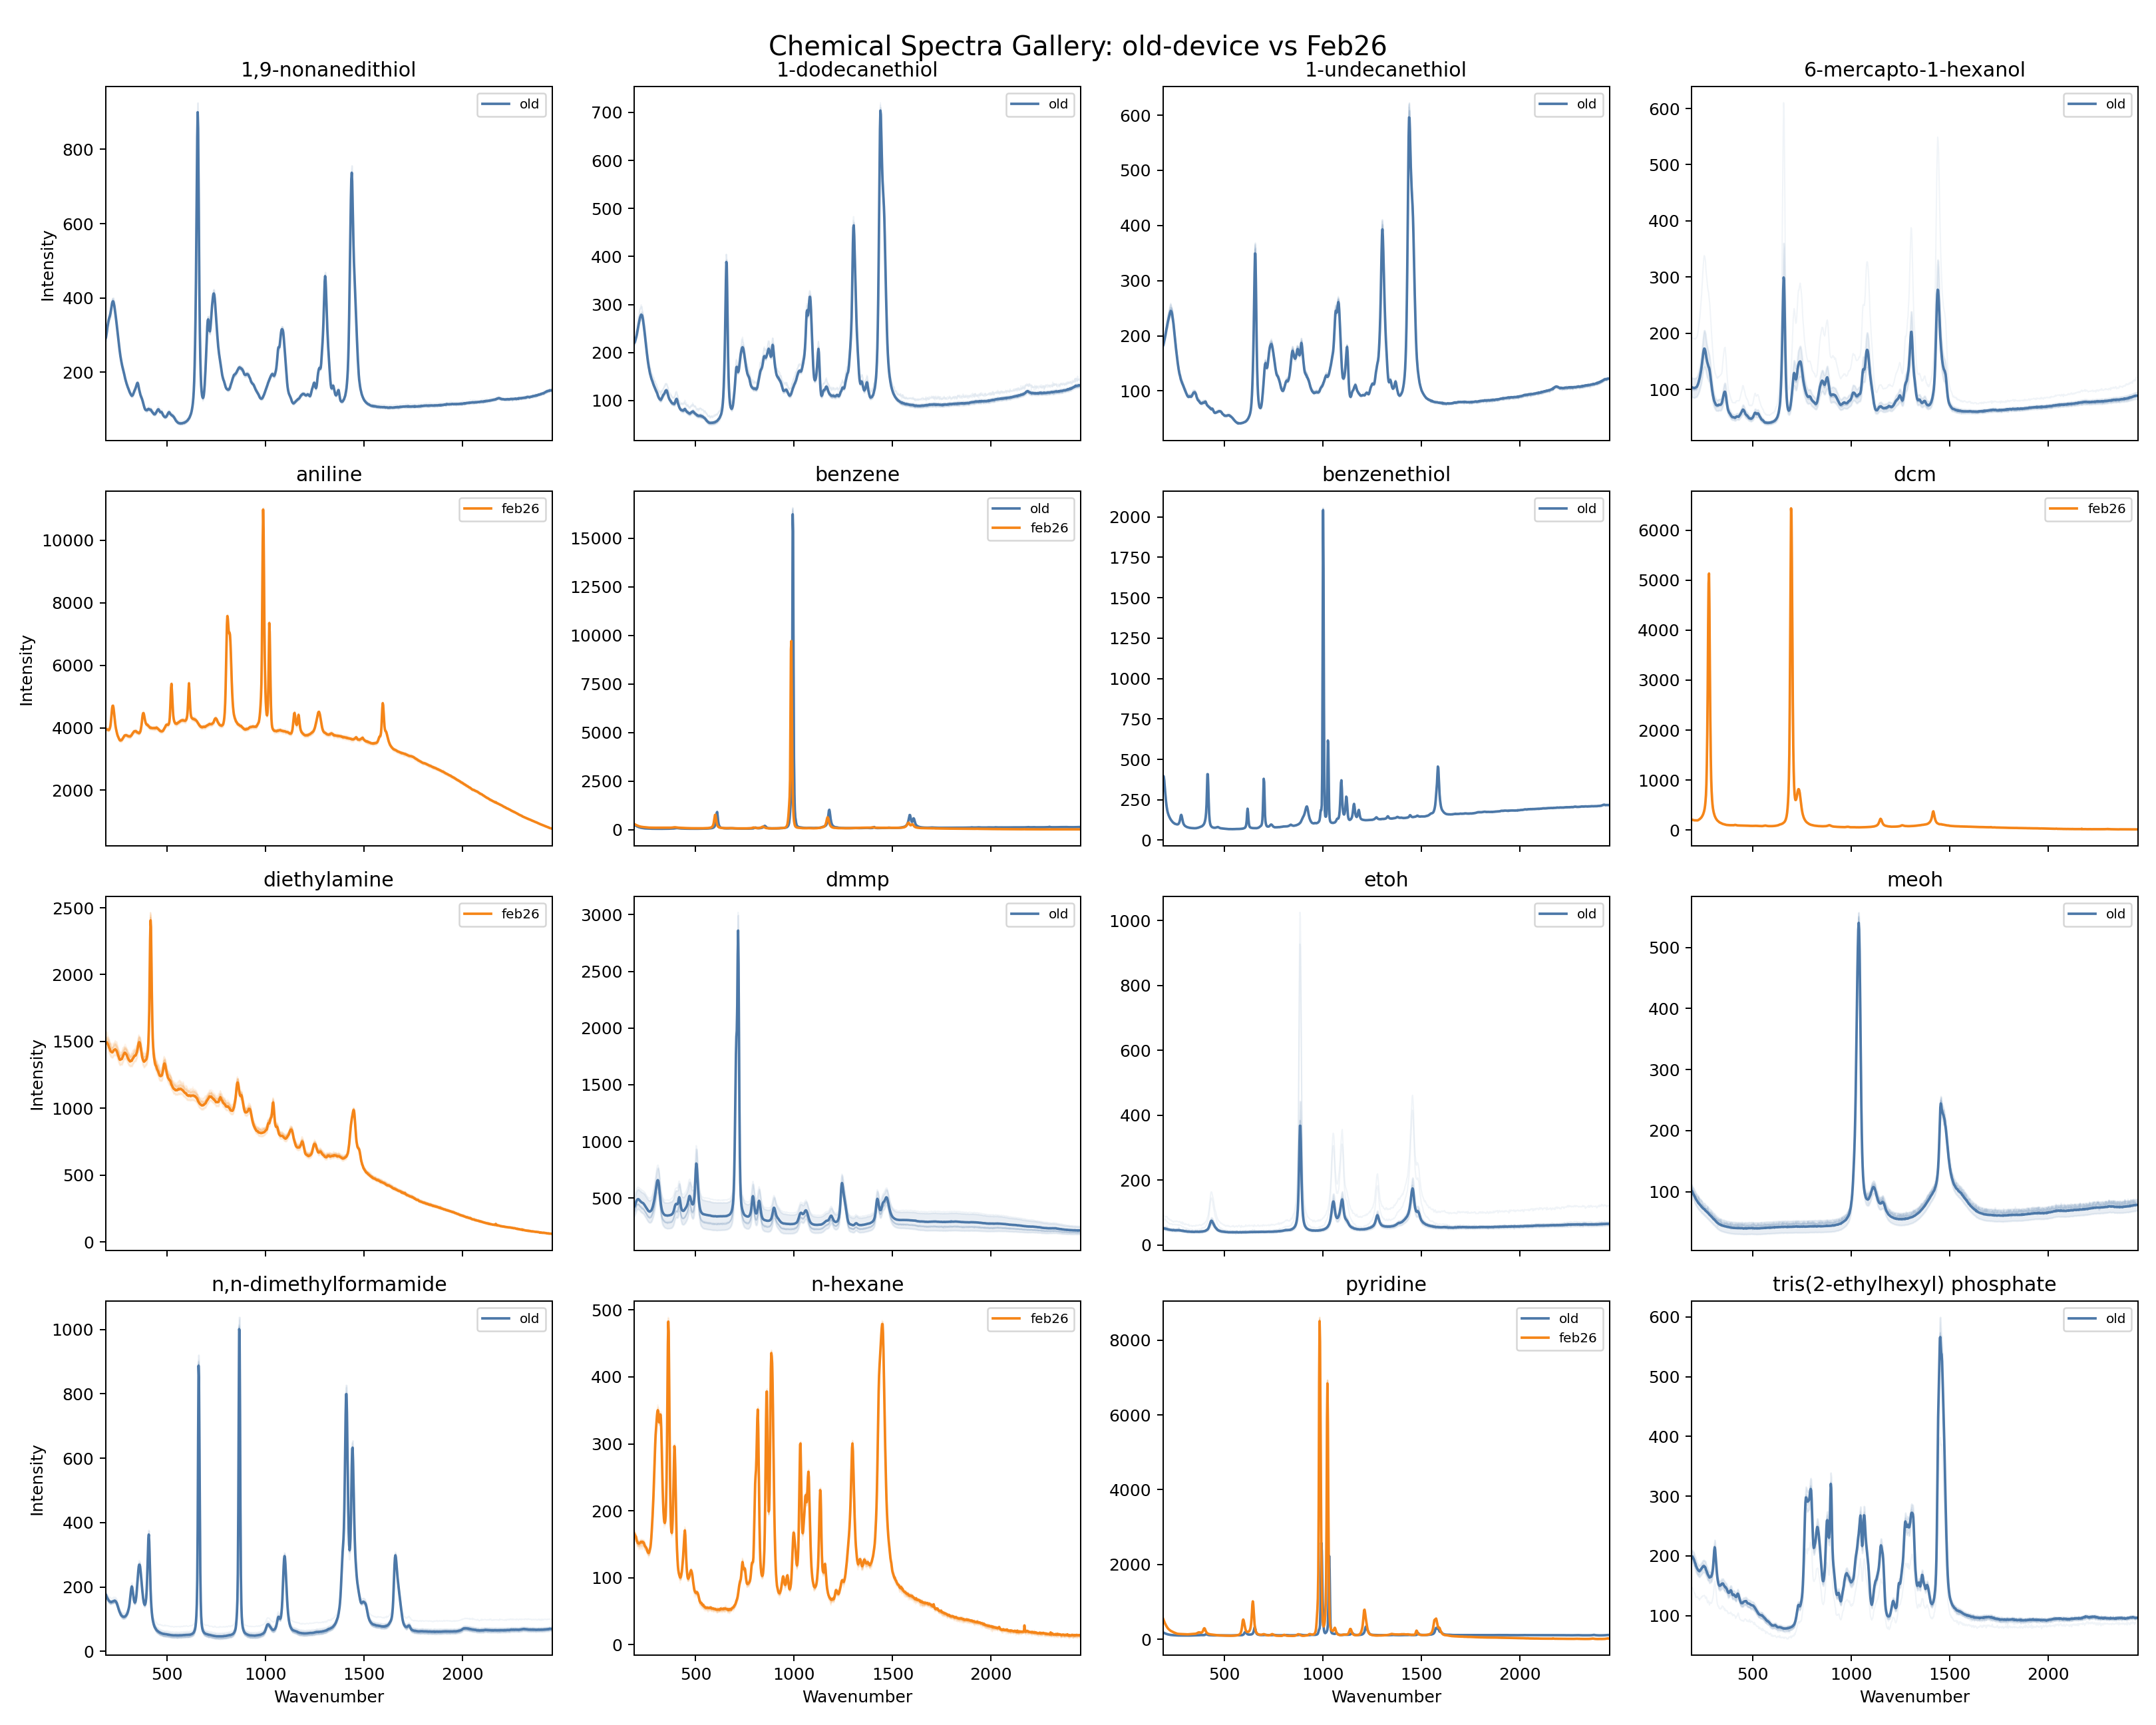
\includegraphics[width=\linewidth]{../figures/chemical_spectra_gallery.png}
    \end{column}
  \end{columns}
\end{frame}

\begin{frame}{1. Closed-Set Extension Results}
  \centering
  \small
  \begin{tabular}{lccc}
    \toprule
    Query subset & Count & Top-1 acc. & Top-2 acc. \\
    \midrule
    Expanded full query set & 765 & 1.000 & 1.000 \\
    Original-label subset & 669 & 1.000 & 1.000 \\
    Feb.\ 26 subset & 200 & 1.000 & 1.000 \\
    True new labels only & 96 & 1.000 & 1.000 \\
    \bottomrule
  \end{tabular}

  \vspace{0.8em}
  \begin{itemize}
    \item Interpretation: once one aligned exemplar per new class is added, the frozen embedding is already strong enough for perfect nearest-neighbor classification.
    \item This shows the embedding is chemically informative; it does not yet test open-set rejection.
  \end{itemize}
\end{frame}

\begin{frame}{2. Frozen-Encoder Open-Set Setup}
  \begin{itemize}
    \item Reference remained the original old-device library only.
    \item Known query set: original old-device queries, \(n=565\).
    \item Unknown query set: Feb.\ 26 aniline, DCM, diethylamine, n-hexane, \(n=100\).
    \item Known controls: Feb.\ 26 benzene and pyridine, \(n=106\).
    \item For every query:
    \begin{itemize}
      \item assign nearest reference label
      \item compute nearest embedding distance
      \item accept if distance \(\le t\), reject if distance \(> t\)
    \end{itemize}
  \end{itemize}
\end{frame}

\begin{frame}{How the Open-Set Threshold Was Determined}
  \begin{itemize}
    \item Threshold selection was done by sweeping candidate values over the empirical distance distribution.
    \item Candidates were built from 401 quantiles of all nearest distances from:
    \begin{itemize}
      \item old-device known queries
      \item true unknown Feb.\ 26 queries
    \end{itemize}
    \item For each threshold \(t\), the script computed:
    \begin{itemize}
      \item known-correct-and-accept rate
      \item unknown reject rate
      \item open-set accuracy
      \item balanced accuracy \(= 0.5 \times (\text{known correct \& accept} + \text{unknown reject})\)
    \end{itemize}
    \item The selected operating point was the threshold with:
    \begin{itemize}
      \item highest balanced accuracy
      \item then highest open-set accuracy
      \item then smallest threshold among ties
    \end{itemize}
  \end{itemize}
\end{frame}

\begin{frame}{2. Frozen-Encoder Open-Set Results}
  \begin{columns}[T]
    \begin{column}{0.56\textwidth}
      \small
      \begin{tabular}{lc}
        \toprule
        Metric & Value \\
        \midrule
        Best threshold & 0.14665 \\
        Known correct \& accept & 1.000 \\
        Unknown reject rate & 1.000 \\
        Open-set accuracy & 1.000 \\
        Balanced accuracy & 1.000 \\
        \bottomrule
      \end{tabular}

      \vspace{0.8em}
      Distance summary:
      \begin{itemize}
        \item known mean: 0.00635, known max: 0.04765
        \item unknown mean: 0.42804, unknown min: 0.29514
        \item known-control mean: 0.16965
      \end{itemize}
    \end{column}
    \begin{column}{0.44\textwidth}
      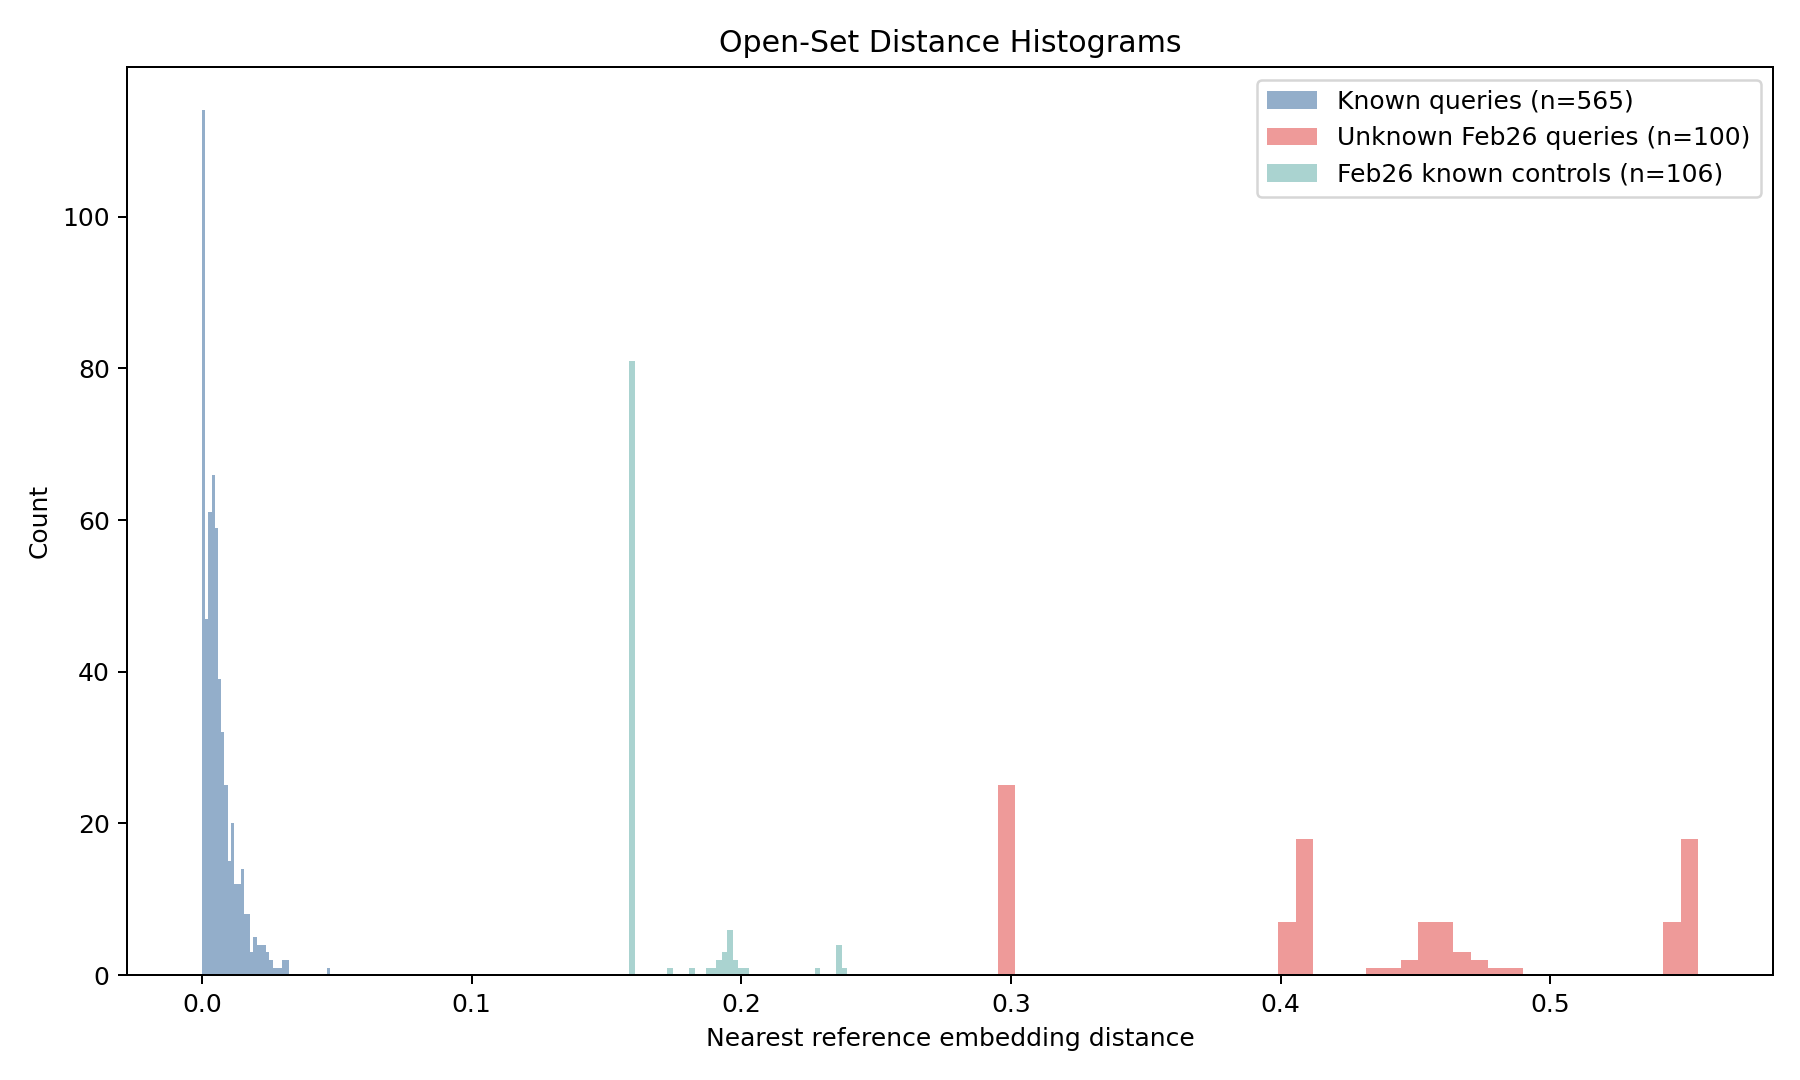
\includegraphics[width=\linewidth]{../figures/open_set_distance_histograms.png}
    \end{column}
  \end{columns}
\end{frame}

\begin{frame}{2. Interpretation of the Frozen-Encoder Result}
  \begin{columns}[T]
    \begin{column}{0.52\textwidth}
      \begin{itemize}
        \item The threshold looks perfect only on the old-known vs true-unknown split.
        \item There is a wide empty gap between:
        \begin{itemize}
          \item old known max distance: 0.04765
          \item unknown min distance: 0.29514
        \end{itemize}
        \item The chosen threshold 0.14665 is simply one candidate inside that gap.
        \item Feb.\ 26 benzene and pyridine expose the real failure:
        \begin{itemize}
          \item top-1 class remained correct for both
          \item but both were rejected at 100\%
        \end{itemize}
        \item So the issue was not class confusion. It was device-shifted distance inflation.
      \end{itemize}
    \end{column}
    \begin{column}{0.48\textwidth}
      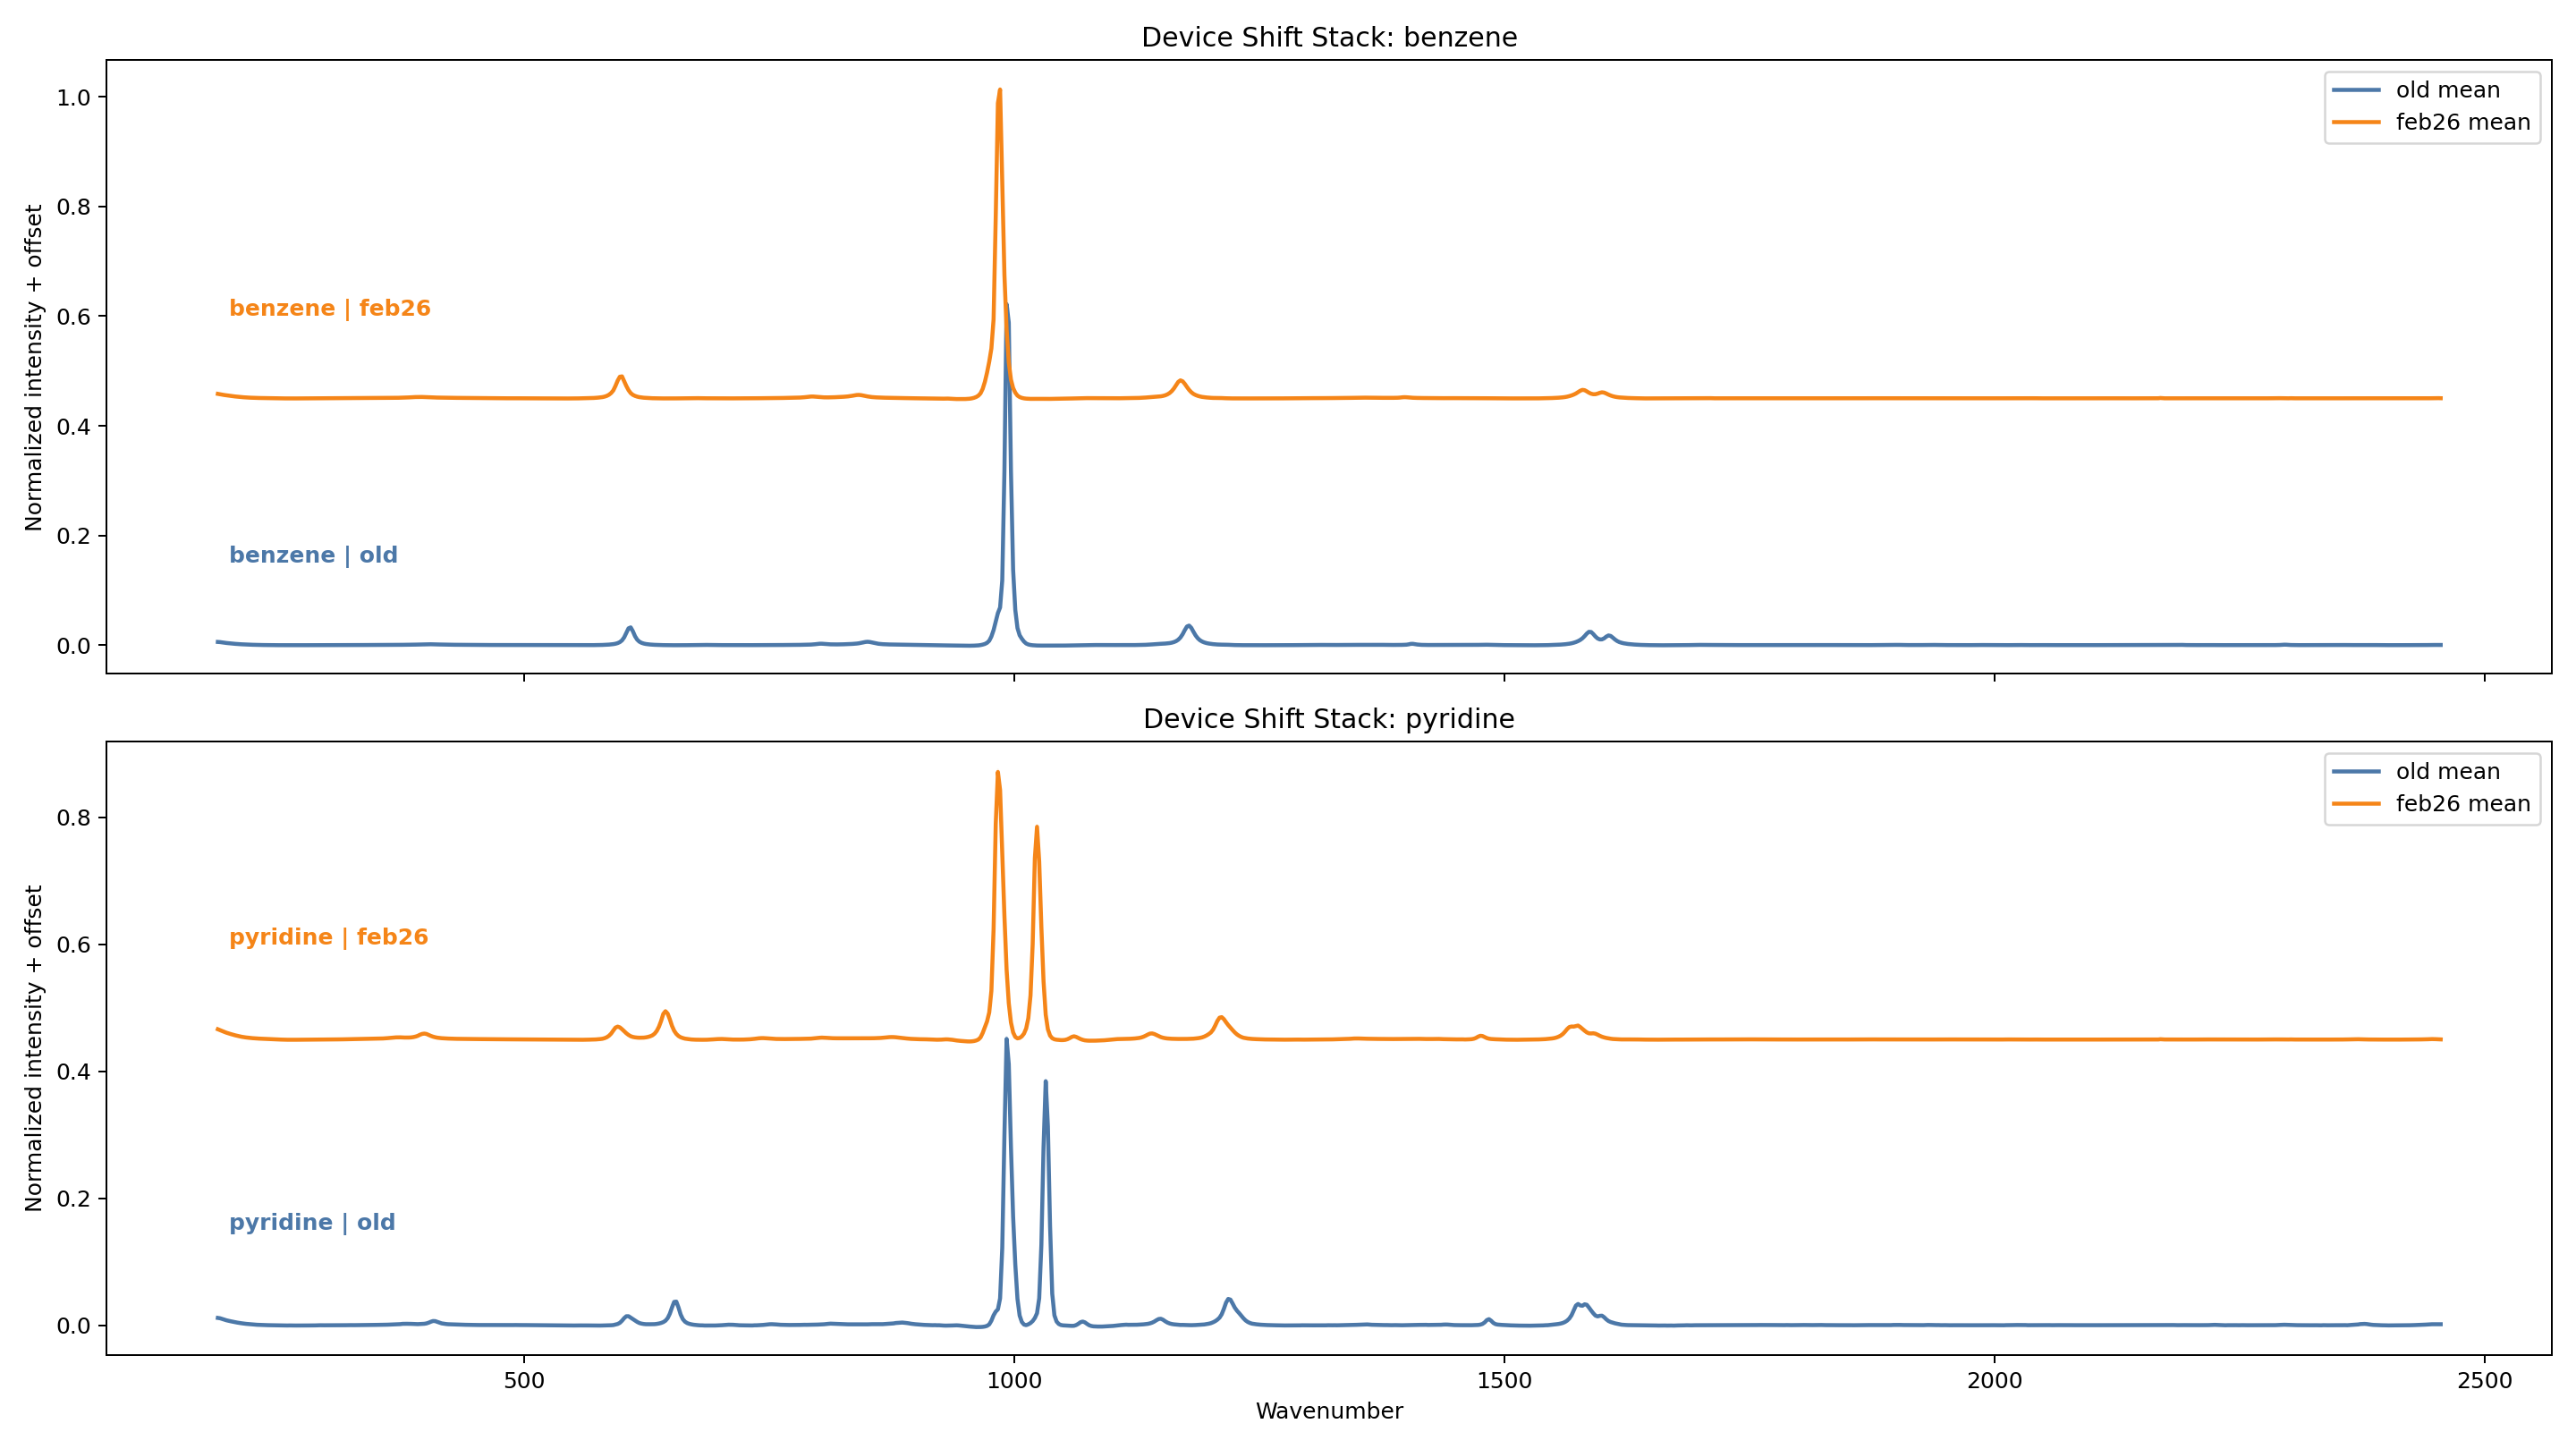
\includegraphics[width=\linewidth]{../figures/device_shift_stacked_spectra.png}
    \end{column}
  \end{columns}
\end{frame}

\begin{frame}{3. Threshold Recalibration Without Retraining}
  \begin{itemize}
    \item The same frozen encoder was kept.
    \item The threshold sweep was repeated, but the known pool now included both:
    \begin{itemize}
      \item original old-device known queries
      \item Feb.\ 26 benzene and pyridine controls
    \end{itemize}
    \item New best threshold: 0.23911.
  \end{itemize}

  \vspace{0.5em}
  \small
  \begin{tabular}{lcc}
    \toprule
    Quantity & Frozen threshold & Recalibrated threshold \\
    \midrule
    Best threshold & 0.14665 & 0.23911 \\
    Unknown reject rate & 1.000 & 1.000 \\
    Benzene reject rate & 1.000 & 0.000 \\
    Pyridine reject rate & 1.000 & 0.040 \\
    \bottomrule
  \end{tabular}

  \vspace{0.8em}
  \begin{itemize}
    \item Interpretation: the baseline embedding was mostly usable; the threshold was under-calibrated for cross-device knowns.
  \end{itemize}
\end{frame}

\begin{frame}{4. Cross-Device Fine-Tuning Setup}
  \begin{itemize}
    \item Fine-tuning used the pretrained encoder as initialization.
    \item Added cross-device training data only for overlapping known classes:
    \begin{itemize}
      \item 10 Feb.\ 26 benzene spectra
      \item 10 Feb.\ 26 pyridine spectra
    \end{itemize}
    \item The remaining Feb.\ 26 benzene and pyridine spectra were held out as controls.
    \item All true unknown classes remained fully held out.
    \item Training details:
    \begin{itemize}
      \item contrastive loss on random positive/negative pairs
      \item light augmentation: additive noise and small shifts
      \item 40 epochs, learning rate \(10^{-4}\)
    \end{itemize}
  \end{itemize}
\end{frame}

\begin{frame}{4. Fine-Tuning Results}
  \begin{columns}[T]
    \begin{column}{0.56\textwidth}
      \small
      \begin{tabular}{lc}
        \toprule
        Metric & Value \\
        \midrule
        Best threshold & 0.12122 \\
        Known correct \& accept & 1.000 \\
        Known-control accept & 1.000 \\
        Unknown reject rate & 1.000 \\
        Open-set accuracy & 1.000 \\
        \bottomrule
      \end{tabular}

      \vspace{0.8em}
      Control distances moved inward:
      \begin{itemize}
        \item benzene mean: 0.15930 \(\rightarrow\) 0.07003
        \item pyridine mean: 0.20317 \(\rightarrow\) 0.08792
      \end{itemize}
    \end{column}
    \begin{column}{0.44\textwidth}
      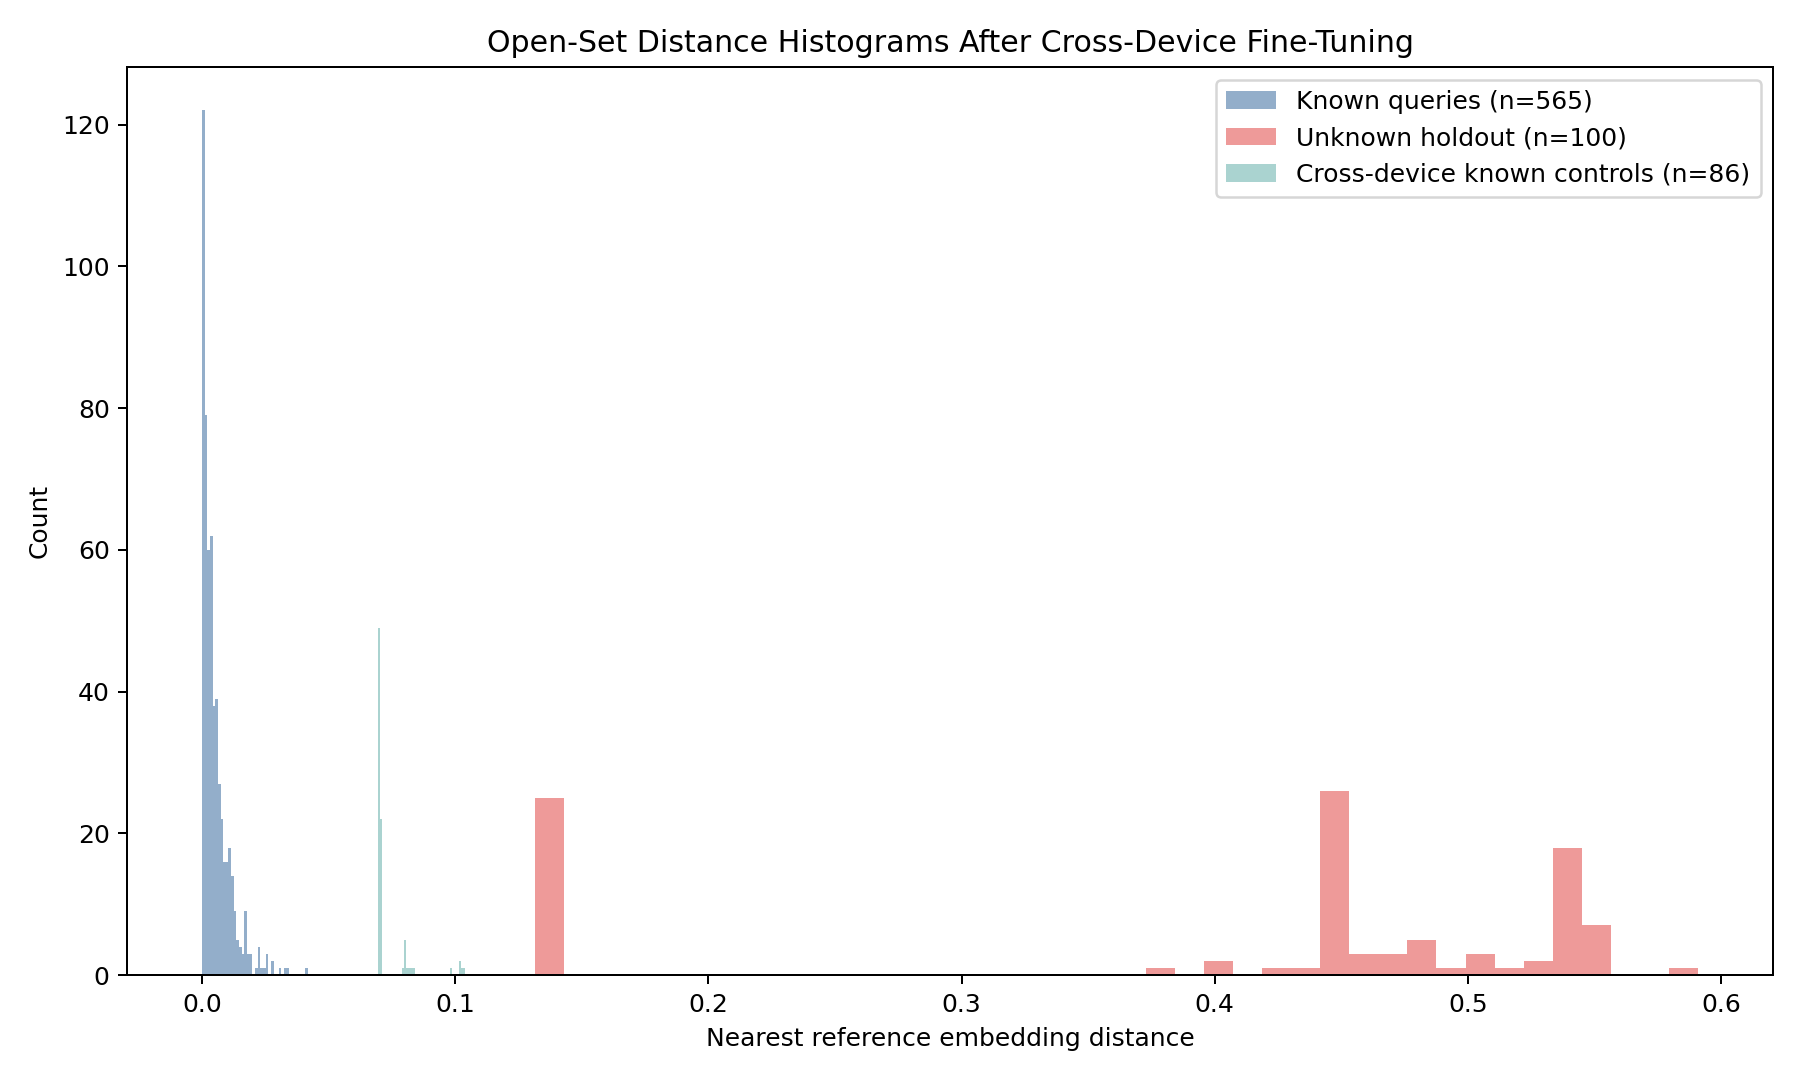
\includegraphics[width=\linewidth]{../figures/open_set_distance_histograms_retrained.png}
    \end{column}
  \end{columns}
\end{frame}

\begin{frame}{Representation-Level Evidence From the Figures}
  \begin{columns}[T]
    \begin{column}{0.5\textwidth}
      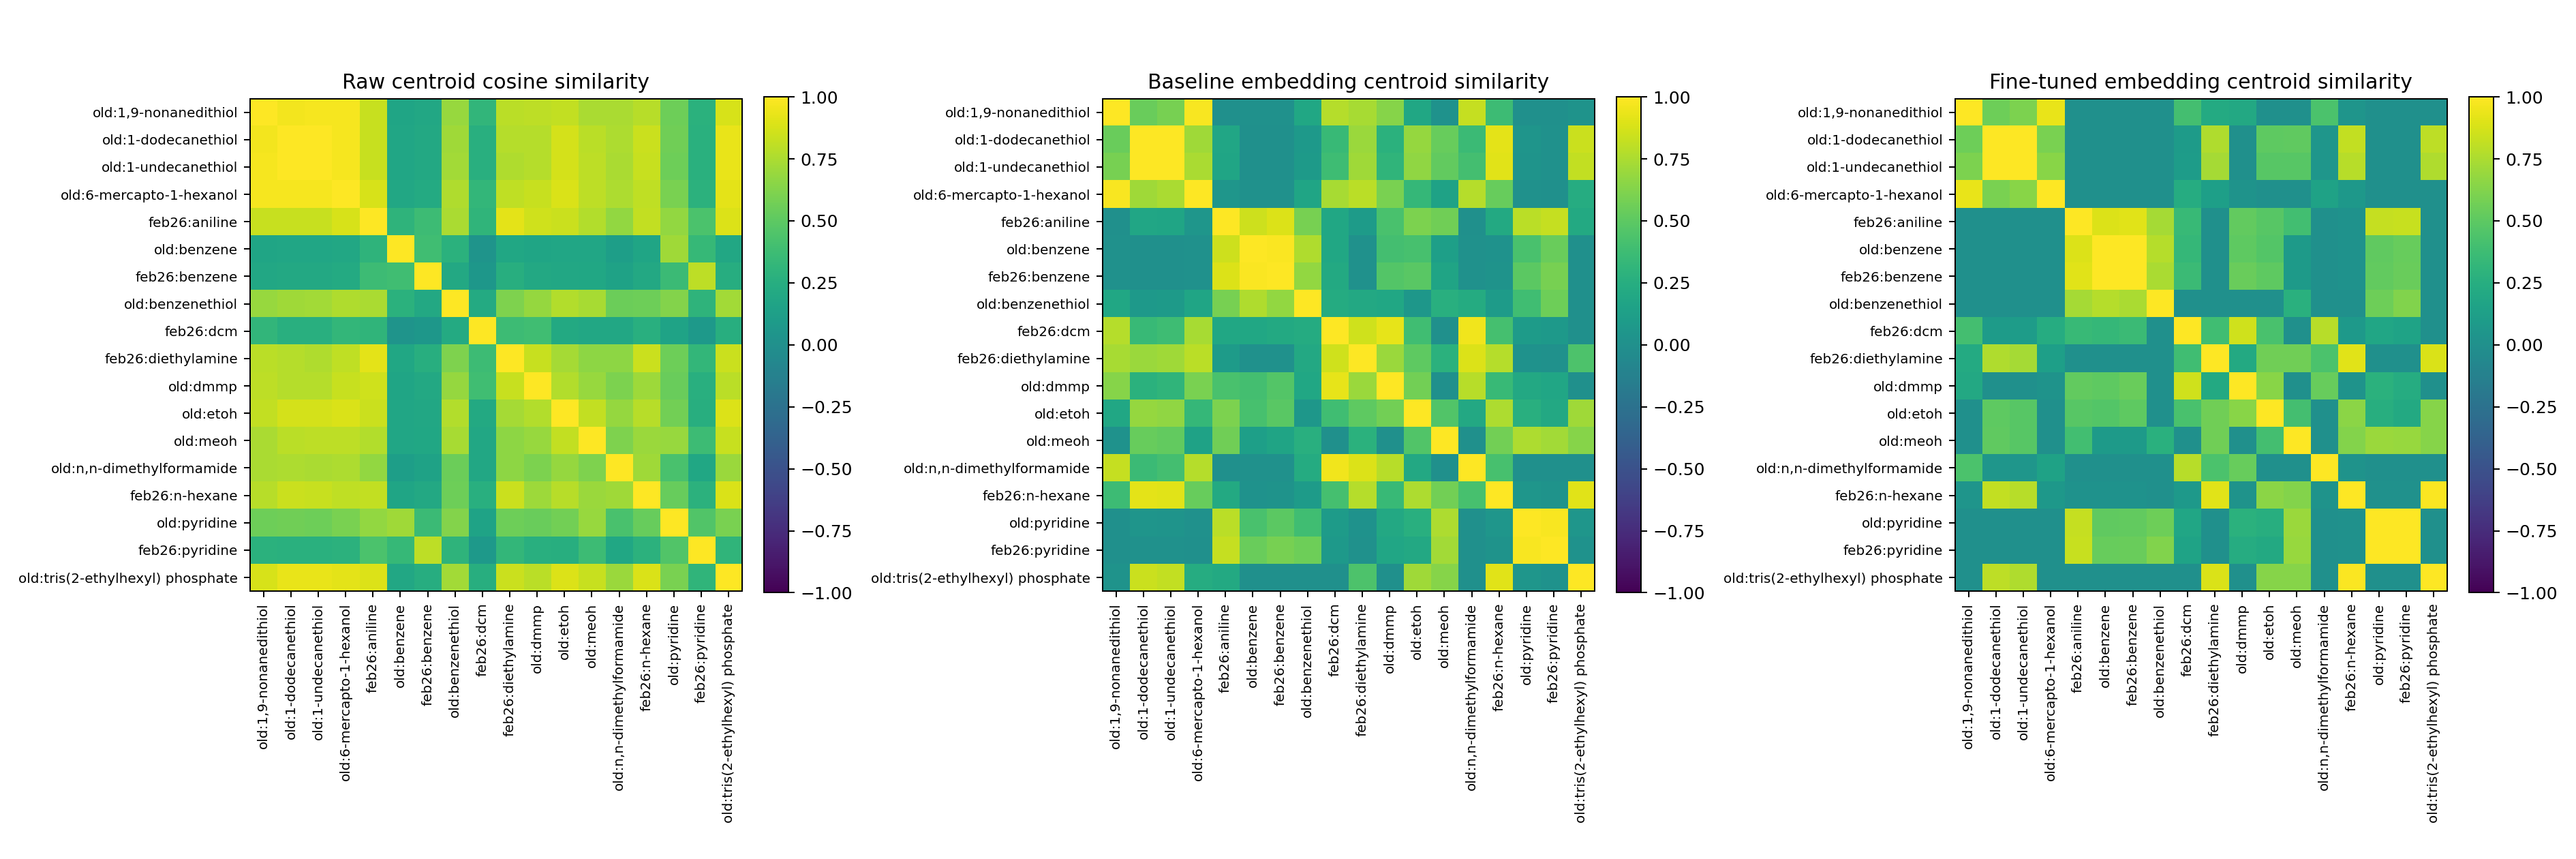
\includegraphics[width=\linewidth]{../figures/centroid_similarity_panels.png}
    \end{column}
    \begin{column}{0.5\textwidth}
      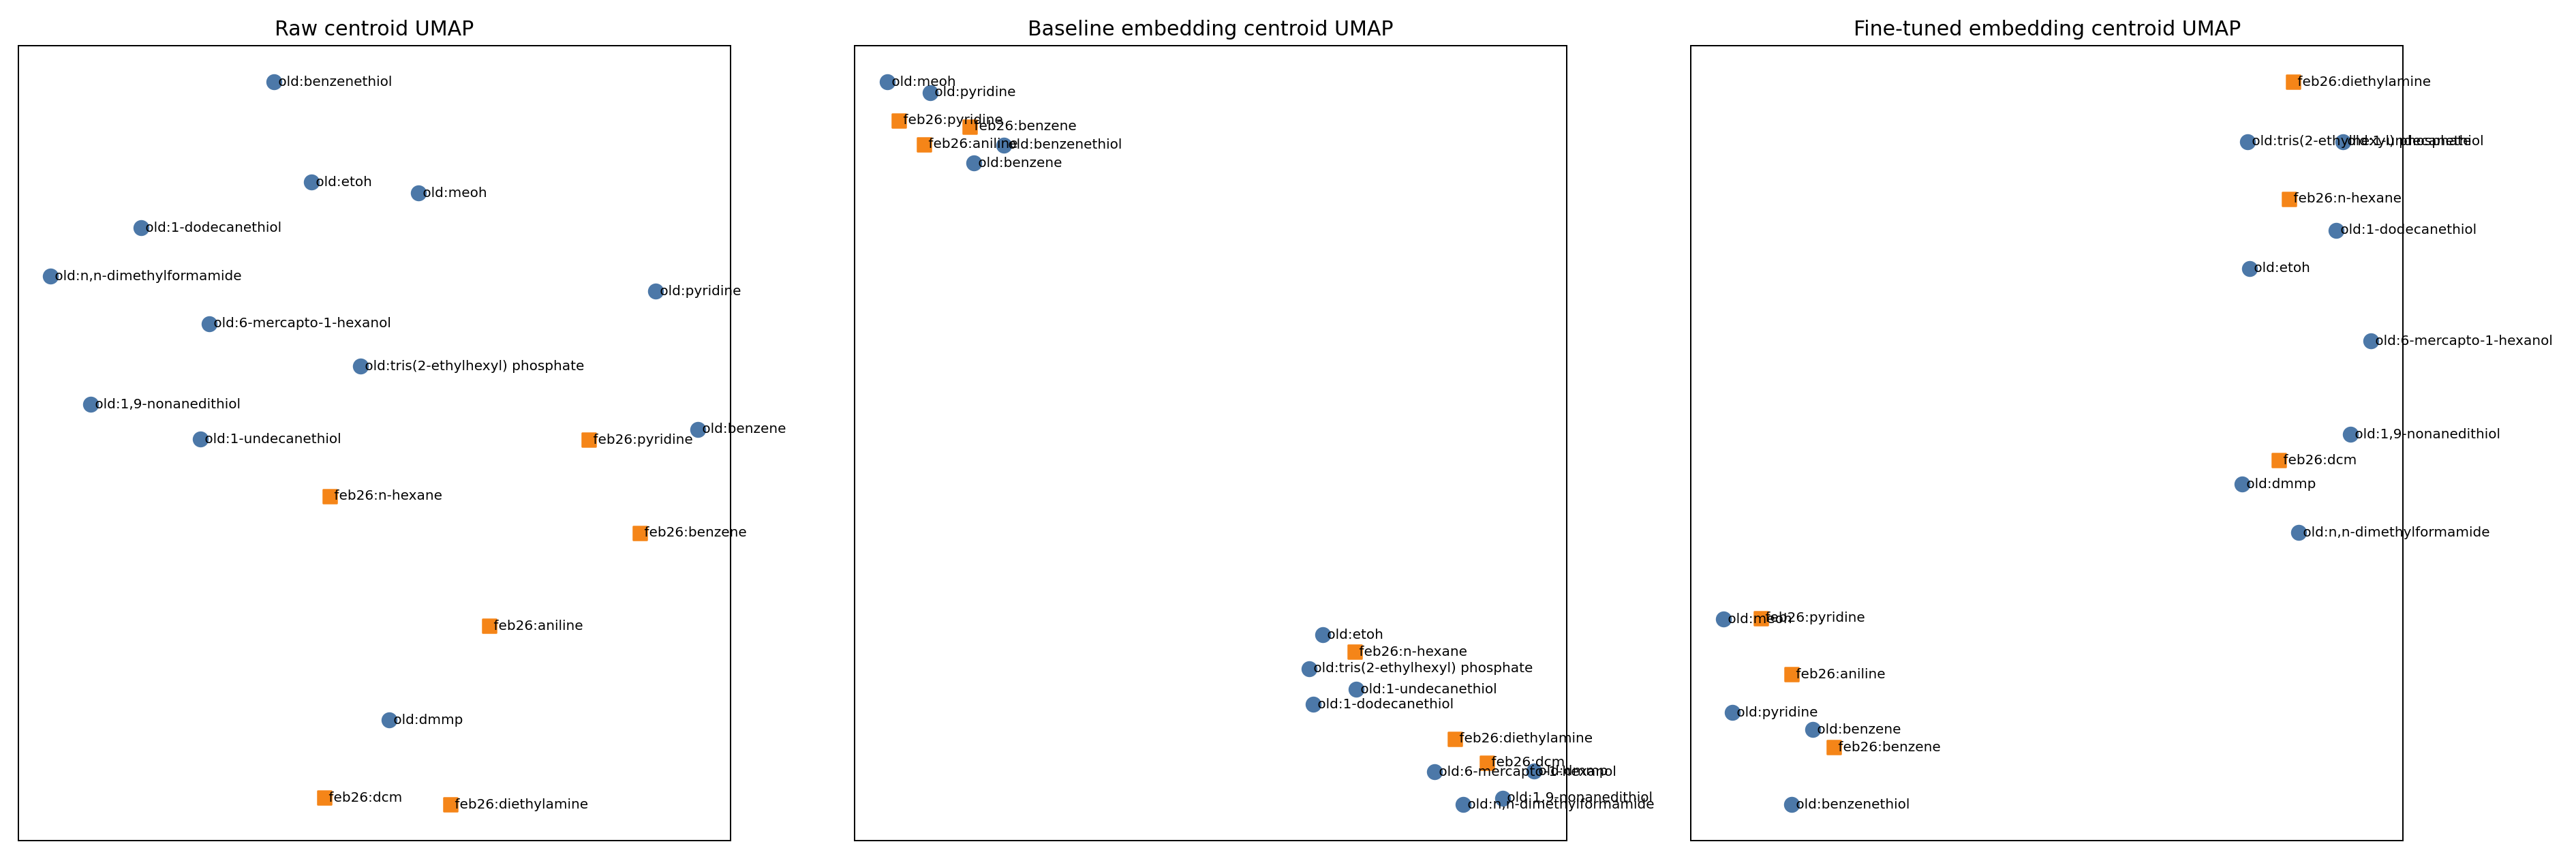
\includegraphics[width=\linewidth]{../figures/centroid_umap_panels.png}
    \end{column}
  \end{columns}

  \vspace{0.5em}
  \small
  Same-chemical cross-device centroid similarity:
  \begin{itemize}
    \item raw space: benzene 0.390, pyridine 0.454
    \item baseline embedding: benzene 0.988, pyridine 0.979
    \item fine-tuned embedding: benzene 0.998, pyridine 0.996
  \end{itemize}
\end{frame}

\begin{frame}{Overall Interpretation}
  \begin{itemize}
    \item The pretrained encoder already captured the right chemical structure.
    \item That is why:
    \begin{itemize}
      \item closed-set extension worked immediately
      \item benzene and pyridine controls still got the correct nearest label
    \end{itemize}
    \item The main deployment problem was absolute distance calibration across devices.
    \item Recalibration alone recovered most cross-device knowns.
    \item Fine-tuning on overlapping knowns solved the calibration problem more cleanly by pulling same-chemical cross-device embeddings closer together while keeping true unknowns separable.
  \end{itemize}
\end{frame}

\begin{frame}{Key Takeaways}
  \begin{enumerate}
    \item Closed-set library extension is easy here: one aligned exemplar per new class was enough for perfect classification.
    \item Open-set thresholding cannot be trusted if it is calibrated only on one device.
    \item Cross-device known controls are essential; without them, a threshold can look perfect while failing in practice.
    \item The frozen encoder was already good; the bottleneck was mostly cross-device distance shift.
    \item Cross-device fine-tuning on overlapping known classes produced the cleanest operational result.
  \end{enumerate}
\end{frame}

\end{document}
